%%% Document packages
\RequirePackage{fix-cm}                                                                 % Defines a specific font class to use. Fixes bf sc T1 class issue.
\documentclass[a4paper, 12pt]{report}                                          % Defines the type of document to compile.
\usepackage[top=2.5cm,bottom=2.5cm,left=3cm,right=3cm]{geometry}

% HUGE size
\makeatletter
	\newcommand\HUGE{\@setfontsize\Huge{30}{30}}
\makeatother 

% Regular chapter headings
\usepackage{titlesec}
\titleformat{\chapter}[hang]{\vspace{-50pt}\normalfont\huge\bfseries}{\thechapter}{1em}{}                         

% Remove paragraph indents
\usepackage{parskip}

% Microtyping
\usepackage{microtype}

% positioning
\usepackage{eso-pic}

%%% Fancy page setup
\usepackage{lastpage}                                                                   % Has a macro that defines the total number of pages.
\usepackage{fancyhdr}                                                                   % Controls the setup of the page.
\pagestyle{fancy}                                                                       % Defines the usual page setup.
\setlength{\headheight}{15pt}                                                           % Sets the header height to contain the header text.
%\fancyhead[L]{\nouppercase{\rightmark}}
\fancyhead[L]{}                                                 % Overwrites the default header so it's not fully capital.
\fancyhead[R]{\nouppercase{\leftmark}}                                                  % Overwrites the default header so it's not fully capital.
\fancyfoot[C]{}                                                                         % Set the center of the  to be empty.
\fancyfoot[R]{\thepage\ of\ \pageref*{LastPage}} % Page number counter. 
\renewcommand{\headrulewidth}{0.4pt}                                                    % Sets the default header underline thickness.
\renewcommand{\footrulewidth}{0.4pt}                                                    % Sets the default footer overline thickness.
\renewcommand{\chaptermark}[1]{\markboth{\thechapter.\ #1}{}}                           % Changes fancyheader[R] to "<Chapter Number>. <Chapter Title>" from "CHAPTER <Chapter Number>. <CHAPTER TITLE>". This saves space and looks nicer.
\renewcommand{\sectionmark}[1]{\markright{\thesection.\ #1}}                            % Changes fancyheader[L] to "<Section Number>. <Section Title>" from "<Section Number>. <SECTION TITLE>". This saves space and looks nicer.

%% Note to the user
% In order to get a single sided document, you need to remove the `twoside` option from the documentclass command, and the [options] in line 14 need to be changed from [LE,RO] to [R].

\fancypagestyle{plain}{\fancyhead{}\fancyhead[R]{\nouppercase{\leftmark}}}              % Whenever a new .tex file or chapter or page is included, the report class defaults to a plain page style. This changes the plain page style using fancyhdr to the style "fancy" defined above. Changes can be made in the second parameter.
\fancypagestyle{declaration}{\fancyhead{}\fancyhead[R]{}}                    % Define adjustments for the declaration page(s).
\fancypagestyle{abstract}{\fancyhead{}\fancyhead[R]{}}                          % Define adjustments for the abstract page(s).
\fancypagestyle{is}{\fancyhead{}\fancyhead[R]{}}                        % Define adjustments for the impact statement page(s).
\fancypagestyle{dedication}{\fancyhead{}\fancyhead[R]{}}                      % Define adjustments for the dedication page(s).
\fancypagestyle{acknowledgements}{\fancyhead{}\fancyhead[R]{}}          % Define adjustments for the acknowledgements page(s).
\fancypagestyle{glossary}{\fancyhead{}\fancyhead[R]{}}                 % Define adjustments for the glossary page(s).
\fancypagestyle{toc}{\fancyhead{}\fancyhead[R]{}}                               % Define adjustments for the table of contents page(s).
\fancypagestyle{lof}{\fancyhead{}\fancyhead[R]{}}                        % Define adjustments for the list of figures page(s).
\fancypagestyle{loa}{\fancyhead{}\fancyhead[R]{}}                     % Define adjustments for the list of algorithms page(s).
\fancypagestyle{lot}{\fancyhead{}\fancyhead[R]{}}                         % Define adjustments for the list of tables page(s).

%%% Text packages
\usepackage[english]{babel}                                                             % Selects the language rules.
%\usepackage[utf8]{inputenc}                                                             % Translates input encodings into LaTeX script. This doesn't work with LuaLaTeX which is my compiler of choice. This may be required for pdfLaTeX, which is Overleaf's default.
\usepackage[T1]{fontenc}                                                                % Selects font encoding.
\usepackage{textcomp}                                                                   % Supports companion fonts.
\usepackage{pdflscape}                                                                  % Arranges PDF landscapely.
\usepackage{afterpage}                                                                  % Deals with pdflscape package issues.
\usepackage{siunitx}                                                                    % Deals with unit formatting.
\usepackage{lmodern} \normalfont                                                               % Fixes the bf sc T1 class issue.
\DeclareFontShape{T1}{lmr}{b}{sc}{<->ssub*cmr/bx/sc}{}                                  % Fixes the bf sc T1 class issue.
\DeclareFontShape{T1}{lmr}{bx}{sc}{<->ssub*cmr/bx/sc}{}                                 % Fixes the bf sc T1 class issue.
%\usepackage{helvet} \renewcommand{\familydefault}{\sfdefault}                          % Sets the font to Helvettica.
%\usepackage{fontspec} \setmainfont{Arial}                                              % Sets the font to Arial.
\usepackage{setspace}                                                                   % Customizes line spacing.
%\onehalfspacing{}                                                                      % Use one and a half spacing.
%\doublespacing{}                                                                       % Use double spacing.

%% Note to the user
% The UCL guidelines suggest that ("should") the lines should be 1.5x or 2x spaced. Uncomment (remove the corresponding "%" before the line) to use (line 48 for 1.5x spacing, 49 for 2x spacing).
% The UCL guidelines enforce that ("must be") margins at the binding edge must be not be less than 40 mm (1.5 inches) and other margins not less than 20 mm (.75 inches). In this document, both left and right margins are set to 40mm, and top and bottom to 20mm. If the user wants just the binding edge to be 40mm, and the other to be 20mm (or more), they should change the "right" parameter of the geometry package options (line 4).
% The UCL guidelines suggest that ("recommend") the minimum font size is 12. This can be changed in the \documentclass [options] selection (line 3). In this document, the default to 12pt.
% The UCL guidelines suggest that ("recommend") the font is either Arial or Helvettica. I have included ways of using those fonts in the document above, uncomment to use. (line 45 for Helvettica, 46 for Arial).
% The Arial font does not ship by default with Linux distros. In order to get this font on Linux (if compiling locally, Overleaf should have this as default), use the following commands:
% wget http://www.itzgeek.com/msttcore-fonts-2.0-3.noarch.rpm
% rpm -Uvh msttcore-fonts-2.0-3.noarch.rpm
% The last command will likely need to be run as admin (using sudo). The -Uvh option updates the package if available, installs otherwise.
% The margins have been set using the geometry package options. I have selected the margins to be as narrow as possible to comply with the guidelines, but this can be changed.

%%% Bibliography packages
\usepackage[style=authoryear-comp,sorting=nyt,url=true,arxiv=abs,nohashothers=false, backend=biber, natbib=true, backref=true, dashed=false, isbn=false, eprint=false, date=year, maxcitenames=2, maxbibnames=99, uniquename=false, uniquelist=false]{biblatex} % Controls the bibliography style and sorting.

% Add line between references
\setlength\bibitemsep{\baselineskip}
% Imports the bibliography.
\addbibresource{references.bib}  
\usepackage{xurl}                                                     

% Links
\usepackage{hyperref}
\hypersetup{
	colorlinks=true,
	linkcolor=blue,
	filecolor=blue,      
	urlcolor=blue,
	citecolor=blue,
	pdftitle={MSc Thesis},
	pdfauthor={Rory Creedon},
}

\DefineBibliographyStrings{english}{%
	backrefpage = {Cited on page},% originally "cited on page"
	backrefpages = {Cited on pages},% originally "cited on pages"
}

%%% Custom referencing commands
\newcommand{\secref}[1]{Sec.\ \ref{#1}}                                                 % Creates a reference to a section as Sec. [].
\newcommand{\equatref}[1]{Eq.\ \eqref{#1}}                                              % Creates a reference to a section as Eq. [].
\newcommand{\tabref}[1]{Table\ \ref{#1}}                                                % Creates a reference to a section as Table [].

%%% Math packages
\usepackage{amsmath, amssymb, amsthm}                                                           % Defines tools required for math mode.
\usepackage{bbm}
\usepackage{amsfonts}                                                                   % Defines extended font set for math mode.
%\usepackage{bm}                                                                        % Makes math symbols bold in math mode.
\usepackage{eucal}                                                                      % Allows for mathcal typesetting. 
\usepackage{breqn}                                                                      % Can split equations over multiple lines, allows for $$ with inline math.
\numberwithin{equation}{section}

%%% Image packages
\usepackage{graphicx}                                                                   % Enhanced graphics support.
\usepackage{float}                                                                      % Improves figure and table positioning.
\usepackage{caption}                                                                    % Custom captions (orientations mainly).
\usepackage{csquotes}                                                                   % Advanced inline and display quotations.
\usepackage{subcaption}                                                                 % Applies for subfigures.
\usepackage{rotating}                                                                   % Allows figures to be rotated.
\usepackage[export]{adjustbox}

%%% Image listing directory
\graphicspath{{Figures/}}                                                               % Sets the directory of the images so document structure is tidier.

%%% Feynman diagram package
%\usepackage[compat=1.1.0]{tikz-feynman}                                                 % Can define and use Feynman diagrams. Note - if this is not compiling well using pdfLaTeX use LuaLaTeX.

%%% Text packages
\usepackage{multicol}                                                                   % Allows multiple columns to be used.
\usepackage{gensymb}                                                                    % Provides generic commands for both text and math modes, like celsius, degree etc.
\usepackage{listings}                                                                   % Provides source code in LaTeX, which is not processed. 

%%% rithm packages
%\usepackage[ruled,vlined]{algorithm2e}                                                  % Imports a framework for defining algorithms.
\usepackage{algorithm}
\usepackage{algpseudocode}

%%% Table packages
\usepackage{ltablex}                                                                    % Combines longtable (multi-page tables with varying geometric properties) into tabularx environments.
\usepackage{makecell}                                                                   % Allows splitting a single cell over many rows using \makecell.
\usepackage{multirow}                                                                   % Allows multiple rows to be combined in a table.
%\usepackage{multicolumn}                                                               % Allows multiple columns to be combined in a table.
\usepackage{tabularx}                                                                   % Creates tables that can use the alignment as is needed.
\usepackage{booktabs}                                                                   % Creates better quality tables.

\usepackage{mathtools}

%Referencing
% Referencing
\usepackage{cleveref}
\newtheorem{proposition}{Proposition}

%%% Document development
\usepackage[color=blue!40, textwidth=25mm]{todonotes}   
                                           % used to annotate the documents and make notes about what needs doing and what doesn't.
\newcommand{\comment}[1]{\todo[size=\tiny]{#1}}

%%% Replacement fields
% Note - make sure that you use the space command `\ ` between each word here. newcommand treats spaces in the definitions as terminations.
\newcommand{\authorName}{\textbf{Rory Creedon}}                                         % Replace the \textbf command and its contents with your name.
\newcommand{\primarySupervisor}{Colin Rowat}                           % Replace the \textbf command and its contents with the name of your primary supervisor.
\newcommand{\secondarySupervisor}{Matthew Caldwell}                       % Replace the \textbf command and its contents with the name of your secondary supervisor.
\newcommand{\examiningCommittee}{\textbf{EXAMINING COMMITTEE}}                         % Replace the \textbf command and its contents with the name of the examining comittee.
\newcommand{\wordCount}{\textbf{WORD COUNT}}                                           % Replace the \textbf command and its contents with the word count.
\newcommand{\submissionDate}{\textbf{11\textsuperscript{th} September 2023}}                                 % Replace the \textbf command and its contents with the submission date.
\newcommand{\thesisTitle}{\textbf{Learning from Revealed Algorithmic Recourse Preferences}}                                      % Replace the \textbf command and its contents with the title of your thesis.
\newcommand{\department}{Department of Computer Science}                                        % Replace the \textbf command and its contents with the name of your department.
\newcommand{\signatureFile}{example-image-a}                                            % Replace the \textbf command and its contents with the directory of the image of your signature.

% Argmin and argmax
\DeclareMathOperator*{\argmin}{argmin}
\DeclareMathOperator*{\argmax}{argmax}
\DeclareMathOperator*{\argsort}{\texttt{argsort}}
\DeclareMathOperator*{\softsort}{\texttt{SoftSort}}
\DeclareMathOperator*{\cost}{\texttt{cost}}
\newcommand{\baseline}{\rule{0pt}{3ex}$\hat{\beta} = \beta^{\text{U}}$, $\hat{W} = I$}

% Section level equation numbering
\numberwithin{equation}{section}

\begin{document}
%\pagenumbering{arabic}

% 0a Title
\begin{singlespace}
    \begin{titlepage}
        %Include the logo
        \center{}
        
\includegraphics[width=0.75\linewidth]{Title/logo.png} \vspace{0.5cm}

        %Include the thesis title
        \rule{\linewidth}{0.5mm} \\[0.4cm]
            { \begin{spacing}{1}
            	\huge \bfseries \textsc{\thesisTitle}
              \end{spacing}}
        \rule{\linewidth}{0.5mm} \\[1.5cm]

        %Include the author information
        \LARGE \textbf{\textsc{\authorName}}\\
        \textsc{\Large University College London}\\
        \textsc{\Large \department}\\[2cm]

        {\large Submitted to University College London (UCL) in partial fulfilment of the requirements for the award of the degree of \\ \textit{Master of Science in Data Science and Machine Learning}.}\\[2cm]

        %Include the supervisors and examiners
        {\large Industry supervisor: \primarySupervisor}\\
        {\large Academic supervisor: \secondarySupervisor}\\[2cm]

        %Include the supplementary information
        {\large Submission date: \submissionDate}
    \end{titlepage}
\end{singlespace}

%\newpage
%\clearpage
%\chapter*{Declaration}
%\thispagestyle{declaration}
%\noindent I, \authorName, confirm that the work presented in this thesis is my own. Where information has been derived from other sources, I confirm that this has been indicated in the thesis.
%
%\vspace{3cm}
%\begin{flushright}
%    
\includegraphics[width=3cm,right]{Title/logo.png}
%    \authorName\\
%    London, United Kingdom\\
%    \submissionDate{}
%\end{flushright}



% 0b Abstract
\clearpage
{
    \pagestyle{abstract}
    \chapter*{Abstract}
      As algorithmic decision making systems have become more widely used in the real world, interest in algorithmic recourse, a set of actions an individual can perform in order to obtain a positive outcome from a model, has also increased. This thesis addresses three key issues in the generation of algorithmic recourse. Firstly, in the real world, actions such as increasing income and increasing savings are often applied sequentially, as opposed to simultaneously. To this end, we propose a method to find the optimal \textit{sequence} of actions, making use of differentiable sorting. Secondly, we must take into account \textit{individual} preferences over how easy or difficult it is to change features. Thirdly, we must take into account the causal effects of changing one variable on other variables. To address the second and third issues, we design a novel methodology to learn both individual preferences and causal effects by presenting negatively classified individuals with a series of paired comparisons of different sequences of actions. We evaluate this methodology on synthetic data. Compared to a baseline of no knowledge over user preferences or the casual graph, we find that our methodology leads to less costly recourse.    
    \thispagestyle{abstract}
}
\newpage


% 0c Table of contents
{
	\hypersetup{
		linkcolor=black
	}
	\pagestyle{toc}
	\tableofcontents{}
	\thispagestyle{toc}
}
\clearpage

% Introduction
\chapter{Introduction}

Picture a scenario where, after renting for the last 10 years, you are in the process of buying your first home. You require a mortgage of £300,000. Your salary is £50,000, you have savings of £40,000 (excluding that saved for the deposit) and a credit score of 800\footnote{Assume that this is an Experian credit score, where a score 800 corresponds to a `fair' score, see more details \href{https://www.experian.co.uk/consumer/experian-credit-score.html}{here}.}. You decide to apply for a mortgage with a new digital bank, which promises to instantly provide a decision, through its `AI-powered system'. After entering all your details online, you press `Submit'. A new screen appears, informing you that your mortgage application has been unsuccessful. However, it also informs you that if you can increase your income to £70,000 and increase your savings to £50,000 , you will be approved for the mortgage. These actions you can take in order for your mortgage to be approved are known as \textit{algorithmic recourse}.\\

Algorithmic or automated decision making systems are widely used in the real world, often in high stakes environments, where they have a significant impact on the lives of individuals. Some examples include credit scoring, where classifiers are widely used to approve loans and mortgages \citep{odwyerAreYouCreditworthy2018}, in criminal justice, to assess the risk of re-offending \citep{angwinMachineBias2016} and hiring, where candidate screening and video interviews are often automated \citep{kramerProblemsAIVideo2022}. Algorithmic recourse refers to a set of actions an individual can take to remedy a negative decision made by an algorithmic or automated decision making system.\comment{cite this} For example, in the mortgage approval case, the recourse provided was to increase income and credit score. In a hiring setting, it may involve increasing educational achievements or work experience.\\


Whilst algorithmic decision making is highly prevalent, algorithmic recourse is not as common\comment{cite this}. This is concerning, given that recourse has benefits such as increasing trust in algorithmic systems and aiding individuals' ability to make plans and decisions over time \citep{venkatasubramanianPhilosophicalBasisAlgorithmic2020}. Moreover, algorithmic recourse has been argued to have a legal basis in the EU's General Data Protection Regulation (GDPR), where individuals have a \textit{right to recourse}\comment{check this, not sure if this is true - written in survey paper} \citep{voigtEUGeneralData2017}.\\

Generating algorithmic recourse involves finding a feasible alternative set of actions $\mathbf{x}'$ that results in a minimal cost to the individual, subject to a positive outcome from the classifier $h$. Mathematically, we can formulate the algorithmic recourse problem as follows, where $\mathbf{x}$ are the individual's original features, the classifier is assumed to be a binary classifier $h: \mathbb{R}^D \to \{0,1\}$ and $\mathcal{F}$ represents the set of feasible features values (e.g, if $x_{\text{RACE}}=$ ``Black'', then $x'_{\text{RACE}}=$ ``White'' is not feasible).

\begin{align}
	\mathbf{x}^* = & \argmin_{\mathbf{x}'}  \texttt{cost}(\mathbf{x}, \mathbf{x}') \\ \nonumber
	\text{s.t. } & h(\mathbf{x}') = 1, \\ \nonumber
	& \mathbf{x}' \in \mathcal{F}
\end{align}


These alternative sets of features are often referred to as \textit{counterfactual explanations} - counterfactual features that would have resulted in a positive or more favourable outcome\footnote{This thesis will focus on binary classification problems where there is a positive outcome and a negative outcome. However, the problem naturally extends to multi-class classification, where there are different counterfactual explanations for each class.}. There have been various different methods proposed to generate counterfactual explanations, which can accommodate different types of classifiers (e.g., linear models, tree-based models, neural networks), which have different feasibility, plausibility and other constraints, which can be used on different types of data (e.g., tabular data, image data) and can be computed using different methods (e.g., gradient descent, integer linear programming, brute force) (see Table 1 in \textcite{karimiSurveyAlgorithmicRecourse2022}).\comment{could more citations here, but survey paper should do fine}\\

One of the key challenges in providing algorithmic recourse is the cost function itself. Given that humans are not able to express their individual costs/preferences mathematically, it a highly non-trivial task to estimate the cost of changing features $\mathbf{x}$ to  $\mathbf{x}'$\comment{cite and explain why this is}. Estimating the cost function is crucial to providing algorithmic recourse, as without a good understanding of the cost of changing features, the recourse provided could be very costly and difficult to achieve. Again consider the scenario where you have unsuccessfully applied for a mortgage on your first home. Imagine that a highly inaccurate cost function has been used to generate recourse and you have been told to increase your income from £50,000 to £80,000 and to increase your savings from £40,000 to £42,500. This may be highly costly, as it is difficult to obtain a 60\% increase in salary, whilst increasing your savings by £2,500 may be comparatively much easier. Another set of features on the classification boundary, is to increase your income to £65,000 and to increase your savings to £55,000. You would consider the second set of features much less costly to achieve than the first. However, due to the poor estimation of your true cost function, you have been provided with recourse that is difficult to achieve.\\

In this thesis, we highlight and propose solutions for three key issues with existing cost functions in the algorithmic recourse literature.

\begin{enumerate}
	\item A set of actions (e.g, increase income to £70,000, increase savings to £50,000) are typically enacted sequentially, as opposed to simultaneously. Costs should consider the order of these actions, as actions (or \textit{interventions}) have downstream (causal) effects on other variables. For example, after obtaining a raise and increasing your income to £70,000, it now becomes much easier to increase your savings to £50,000. This is addressed in chapter \ref{chapter:causal_recourse}.
	
	\item The cost function should take into account user preferences over feature mutability. For example, picture a scenario where an individual is applying for a PhD and is provided with recourse. They are asked to increase their GRE\footnote{The \href{https://www.ets.org/gre.html}{Graduate Record Examination} (GRE) is a standardised test that is an admissions requirement for some Masters and PhD programmes.} quantitative reasoning score and produce more academic work (i.e., published papers). It is likely that increasing your GRE quantitative score is more easily mutable than producing additional published papers, which take considerable time and effort. This is addressed in chapter \ref{chapter:cost_learning}, where a novel human-in-the-loop approach is proposed to learn user preferences.
	
	\item Causal algorithmic recourse requires specification of the underlying Structural Causal Model (SCM). When we intervene on income (by increasing it to £70,000), we use the SCM to evaluate the downstream (causal) effects, such as leading to an increase in savings. The size and form of this effect are dictated by the SCM. It could be a simple linear relationship (such as 40\% of income is savings, so an increase in income of £20,000 leads to an increase in income of £8,000) or a more complex relationship that includes many non-linear and non-convex functions. An incorrectly specified SCM can lead to an incorrect cost function. For the actions (a) increase income to £70,000 and then (b) increase savings to £50,000, if we believe that in the SCM, there is a linear relationship between income and savings where an increase in income of £1 leads to a £0.40 increase in savings, then we assume that after the increase in income, savings are £8,000 higher (original income is £50,000). However, the true relationship is linear, where an increase in income of £1 leads to a £0.20 increase in savings. This means after the increase in come, savings are only £4,000 higher. The true cost of two actions are higher than the estimated cost in the our estimation of the SCM. This problem is also addressed in chapter \ref{chapter:cost_learning}, where human-in-the-loop approach learns an \textit{linear approximation} of the SCM as well as user preferences.
	
	
\end{enumerate}


The structure of the thesis is as follows. Relevant literature is reviewed in chapter \ref{chapter:lit_review}, causal algorithmic recourse and sequential interventions are discussed in chapter \ref{chapter:causal_recourse}, the methodology proposed to learn costs is discussed in chapter \ref{chapter:cost_learning}, results of and discussion of experiments on synthetic data are in chapter \ref{chapter:experiments} and concluding remarks are made in chapter \ref{chapter:conclusion}.\\

The accompanying code to replicate the experiments in the thesis can be found here: \url{https://github.com/rorycreedon/msc_thesis}.











% Literature Review
\chapter{Literature Review}

\section{Algorithmic Recourse}

\subsection{Motivation}
Description of what algorithmic recourse is and why it is important - use of automatic decision making, GDPR \citep{voigtEUGeneralData2017}. Mention psychological factors causing humans to prefer recourse to explanations (\textbf{to find paper(s)}: was mentioned by Ruth Byrne in \href{https://icml.cc/virtual/2021/11705}{ICML panel session}, from 25 minutes onwards).


\subsection{Problem Set-up}
\begin{itemize}
	\item Description of the original set-up and problem - i.e., 
	\begin{equation} \label{eq:recourse_setup}
		 \mathbf{x}^f = \argmax_{\mathbf{x}' \in \mathbf{\mathcal{X}}} f(\mathbf{x}') - c(\mathbf{x},\mathbf{x}')
	\end{equation} 
	\item Description of the causal recourse set-up and problem \citep{karimiAlgorithmicRecourseCounterfactual2021}
	\item Cost and distance functions, actionability of features
\end{itemize}


\subsection{Recourse methods}
Run through methods mentioned in survey paper \citep{karimiSurveyAlgorithmicRecourse2022} and also those implemented in \href{https://carla-counterfactual-and-recourse-library.readthedocs.io/en/latest/recourse.html}{\texttt{CARLA}}.





\section{Strategic Classification}

\subsection{Standard Strategic Classification}


\begin{itemize}
	\item Begin with \textcite{hardtStrategicClassification2016} and explain the set-up as a Stackelberg game with an example.
	
	\item Algorithms proposed for this task include  \textcite{levanonStrategicClassificationMade2021}, \textcite{chenLearningStrategyAwareLinear2020} and \textcite{ahmadiClassificationStrategicAgents2022}. 
	
	\item Mention extensions such as:
	
	\item Where the cost function is completely unknown to the lender \citep{dongStrategicClassificationRevealed2018}
	
	\item Where the response of lenders to the classifier is noisy \citep{jagadeesanAlternativeMicrofoundationsStrategic2021}.
	
	\item Where borrowers do not know the decision rule \citep{ghalmeStrategicClassificationDark2021, bechavodInformationDiscrepancyStrategic2022}.
	
	\item Where the incentives of lender and borrower align (e.g., recommender systems) \citep{levanonGeneralizedStrategicClassification2022}.
	
	\item Where the cost functions are linked by graphs for the borrowers \citep{eilatStrategicClassificationGraph2023}.
	
	\item Where the borrowers act first \citep{nairStrategicRepresentation2022}.
	
	\item Where the borrowers and lenders update at different rates \citep{zrnicWhoLeadsWho2021}.
\end{itemize}

\subsection{Causal Strategic Classification}
A review of the \textit{causal} strategic classification literature, which focuses more on causal identification of features which are strategically manipulated (without causing an improvement in underlying credit `worthiness') and features which causally affect credit `worthiness'.



\section{Revealed Preferences}
A brief primer on axioms of revealed preferences, and on the literature of \textit{learning from revealed preferences}. To briefly discuss:

\begin{itemize}
	\item Original paper by \textcite{beigmanLearningRevealedPreference2006}, where principal issues a list of prices and the agent purchases different quantities of each good. Over time, the principal learns from the different purchase amounts (which are the revealed preferences).
	\item When prices are of goods and budget of the agent are drawn from an unknown distribution \citep{zadimoghaddamEfficientlyLearningRevealed2012, balcanLearningEconomicParameters2014}.
	\item Where the principal is maximising profit \citep{aminOnlineLearningProfit2015, rothWatchLearnOptimizing2016}.
	\item Move onto a more detailed discussion of \textcite{dongStrategicClassificationRevealed2018}.
\end{itemize}


\section{Pairwise Metric Learning}
\begin{itemize}
	\item Start with an introduction of what pairwise metric learning is and key papers.
	\item Move onto specific proposed adaptation/simplification of the learning algorithm proposed in \textcite{canalOneAllSimultaneous2022}.
\end{itemize}


\section{Canonical Datasets}
The canonical datasets used in the algorithmic recourse and strategic classification literature include:

\begin{itemize}
	\item \href{https://archive.ics.uci.edu/dataset/2/adult}{\texttt{Adult}} - dataset to predict whether someone earns over \$50,000 or more.
	\item \href{https://archive.ics.uci.edu/dataset/144/statlog+german+credit+data}{\texttt{German Credit}} - dataset identifies people as either good or bad credit risks.
	\item \href{https://community.fico.com/s/explainable-machine-learning-challenge}{\texttt{FICO-HELOC}} - dataset of HELOC applications, where applicants have applied for a credit line between \$5,000 and \$150,000. Outcome variable is whether they are a good or bad credit risk.
	\item \href{https://www.kaggle.com/datasets/shebrahimi/financial-distress}{\texttt{Finance}} - dataset to predict financial distress for a number of companies. There are several over different time periods for each company.
\end{itemize}





% Causal Algo Recourse
\chapter{Causal Algorithmic Recourse} \label{chapter:causal_recourse}

In the introduction, three problems with cost functions used in the literature were outlined. The first of these was that actions are typically enacted sequentially (e.g., you first increase your income, and then increase your savings). This is important within the \textit{causal} algorithmic setting, where intervening on a variable (e.g, increasing income) has downstream (causal) effects on other variables such as savings. In this chapter, we first motivate \textit{causal} algorithmic recourse, then explore causal algorithmic recourse with soft, as opposed to hard interventions and finally propose a solution to optimise for ordering of sequential interventions when generating recourse.

\section{Motivation}

As discussed in section \ref{section:cost_functions_lit_review}, the cost of changing features is typically modelled as an $\cost(\mathbf{x,x}')=L_p(\mathbf{x} - \mathbf{x}')$ or the total log percentile shift \citep{ustunActionableRecourseLinear2019}. These cost functions fail to take into account the downstream (causal) effects of changing one feature on other features.\\

In order to correctly measure the cost of changing from features $\mathbf{x}$ to $\mathbf{x}'$, we need to be able to evaluate the causal effects of changing one variable on others. For example, if an individual decides not to inquire about a loan for a number of months (which will change the feature ``number of inquiries in the last 6 months'', the cost of decreasing the feature ``number of inquiries in the last 6 months, excluding the last 7 days'' will be very low or zero. However, if a quadratic cost function (or any $L_p$ norm cost function) is used, this will be interpreted as two separate feature changes and the costs of each will be summed. Whilst this simple case can likely be handled by domain expertise, more complex causal relations will exist. Consider an individual obtaining two more credit cards. Whilst this may reduce the cost of increasing ``number of credit cards'', this may also increase the cost of ``monthly credit card payments'' and may have less clear effects (which need not be linear) on other features.\\

The Mahalanobis distance cost function $\texttt{cost}(\mathbf{x}, \mathbf{x}') = (\mathbf{x} -\mathbf{x}')^T\mathbf{M}(\mathbf{x} - \mathbf{x}')$, where $\mathbf{M}$ is a fixed, known, positive semi-definite square matrix \citep{bechavodInformationDiscrepancyStrategic2022}, does allow for changing one feature to affect the cost of changing other features through the off-diagonal elements in $\mathbf{M}$ (see equation \ref{eq:mahalanobis_example} for a worked example). However, the causal effects rely on the changes being made simultaneously. If we first apply a change to $\mathbf{x}_1$ and then to $\mathbf{x}_2$, as shown below. In equations \ref{eq:mahalanobis_step1} and \ref{eq:mahalanobis_step2}, the changes are applied sequentially and there are no causal effects, leading to a total cost of 5. In equation \ref{eq:mahalanobis_step3}, the changes are applied simultaneously and the effect of changing $\mathbf{x}_1$ leads a lower cost of changing $\mathbf{x}_2$, with a total cost of 4. The importance of sequential changes as opposed to simultaneous changes are discussed in section \ref{section:soft_interventions}.

\begin{equation} \label{eq:mahalanobis_step1}
	[1, 0, 0]^T \left[\begin{array}{lllll}
		1 & 0 & 0 \\
		-0.5 & 1 & 0 \\
		0 & 0 & 1
	\end{array}\right] [1, 0, 0]^T = 1^2 + 0^2 + 0^2 = 1
\end{equation}

\begin{equation} \label{eq:mahalanobis_step2}
	[0, 2, 0]^T \left[\begin{array}{lllll}
		1 & 0 & 0 \\
		-0.5 & 1 & 0 \\
		0 & 0 & 1
	\end{array}\right] [0, 2, 0]^T = 0^2 + 2^2 + 0^2 = 4
\end{equation}

\begin{equation} \label{eq:mahalanobis_step3}
	[1, 2, 0]^T \left[\begin{array}{lllll}
		1 & 0 & 0 \\
		-0.5 & 1 & 0 \\
		0 & 0 & 1
	\end{array}\right] [1, 2, 0]^T = 1^2 + 1.5(2) + 0^2 = 4
\end{equation}


\section{Structural Causal Models} \label{section:scms}

To incorporate changing one feature having a causal effect on the cost of changing another feature, we must model the effect of changing the feature $\mathbf{x}_1$ to $\mathbf{x'}_1$ has on changing the feature $\mathbf{x}_2$ to $\mathbf{x'}_2$. Following \textcite{karimiAlgorithmicRecourseCounterfactual2021}, we can model the world using a structural causal model (SCM) to account for downstream effects. The SCM can be defined formally as $\mathcal{M} = \langle\mathbb{U, V, F}\rangle$ capture all the causal relations in the world, where $\mathbb{U}$ represents set of exogenous variables, $\mathbb{V}$ represents the set of endogenous variables (all are a descendant of at least one of the variables in $\mathbb{U}$) and $\mathbb{F}$ represents the set of structural equations which describe how the endogenous variables can be determined from the exogenous variables \citep{pearl2016causal}.

We can illustrate a simple SCM $\mathcal{M}$ with $\mathbb{U} = \{x_1\}$, $\mathbb{V} = \{x_2, x_3, x_4\}$ and structural equations $\mathbb{F}$ are defined in equation \ref{eq:toy_structural_equations}.

\begin{align} \label{eq:toy_structural_equations}
	x_1 & = u_1 & u_1 \sim N(30 , 5) \\ \nonumber %income
	x_2 & = u_2 + 0.5x_1 & u_2 \sim N(20, 10) \\ \nonumber %savings
	x_3 & = u_3 - 0.25x_2 & u_3 \sim \text{Uniform}(0, 20) \\ \nonumber %debt
	x_4 & = \frac{x_3}{x_1} %debt to income ratio
\end{align}


\begin{figure}[!htb]
	\centering
	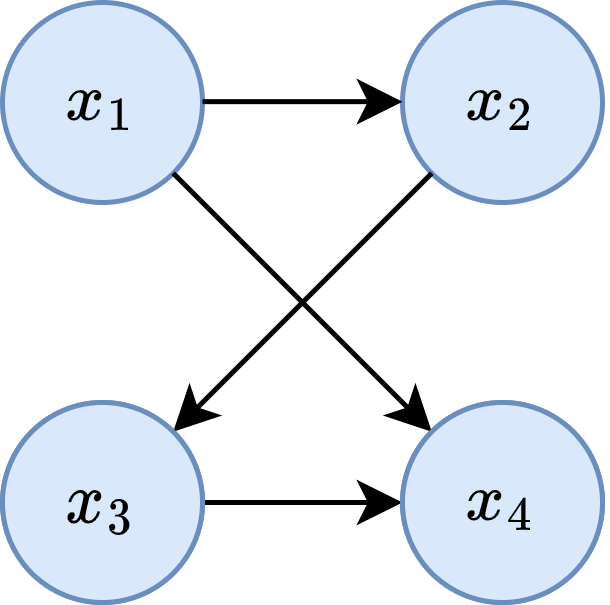
\includegraphics[width=0.25\linewidth]{images/draw.io/Simple SCM.png}
	\caption{Causal graph $\mathcal{G}$ of SCM $\mathcal{M}$.}
	\label{fig:toy_scm}
\end{figure}


The SCM can also be presented with a causal graph $\mathcal{G}$, which is shown in Figure \ref{fig:toy_scm}. Let $x_1$ represent salary (in thousands of pounds), $x_2$ represent savings (in thousands of pounds), $x_3$ represent the debt (in thousands of pounds) and $x_4$ represent debt-to-income ratio. If an individual for whom the SCM $\mathcal{M}$ holds receives an increase in salary, this will lead to an increase in savings and a reduction the debt-to-income ratio. If the individual's initial features were [£30,000, £25,000, £10,000, 1/3]$^T$ and their salary increases to £35,000, then it should then be easier to increase their savings and decrease their debt-to-income ratio than when their salary was £30,000. This toy example shows how the SCM $\mathcal{M}$ encodes the downstream effect of increased salary on both savings and probability of mortgage approval.

[\textbf{DISCUSSION ON PEARL-STYLE DAGS/INBENS CRITIQUE}]

We can use the Abduction-Action-Prediction steps \citep{pearl2016causal} to obtain a \textit{structural counterfactual} of an increase in salary ($x_1$) from £30,000 to £35,000, given that the existing features are [£30,000, £25,000, £10,000, 1/3]$^T$ \comment{go over this example again, should be such that the hard intervention actually leads to the severing of an edge to illustrate the point on hard interventions}

\textbf{1. Abduction}. Calculate the value of exogenous variables before intervention, given the evidence (the current values of the features).

\begin{align}
	u_1 & = x_1 & =  30,000 \\ \nonumber
	u_2 & = x_2 - 0.5x_1 = 25,000 - 0.5(30,00) & = 10,000 \\ \nonumber
	u_3 & = x_3 + 0.25x_2 = 10,000 + 0.25(25,000) & = 16,250
\end{align}

\textbf{2. Action}. Modify the model $\mathcal{M}$ by implementing the intervention on $x_1$ (i.e\., $do(x_2=30,000)$). This leads to a new SCM $\mathcal{M}_1$ where all incoming edges to the intervened upon variable $x_2$ are severed and the value of the intervened upon variable $x_2$ is set to the intervention value £30,000. The resulting SCM $\mathcal{M}_1$ is shown in Figure \ref{fig:toy_scm_severed}, with structural equations $\mathcal{F}_1$.

\begin{figure}[!htb]
	\centering
	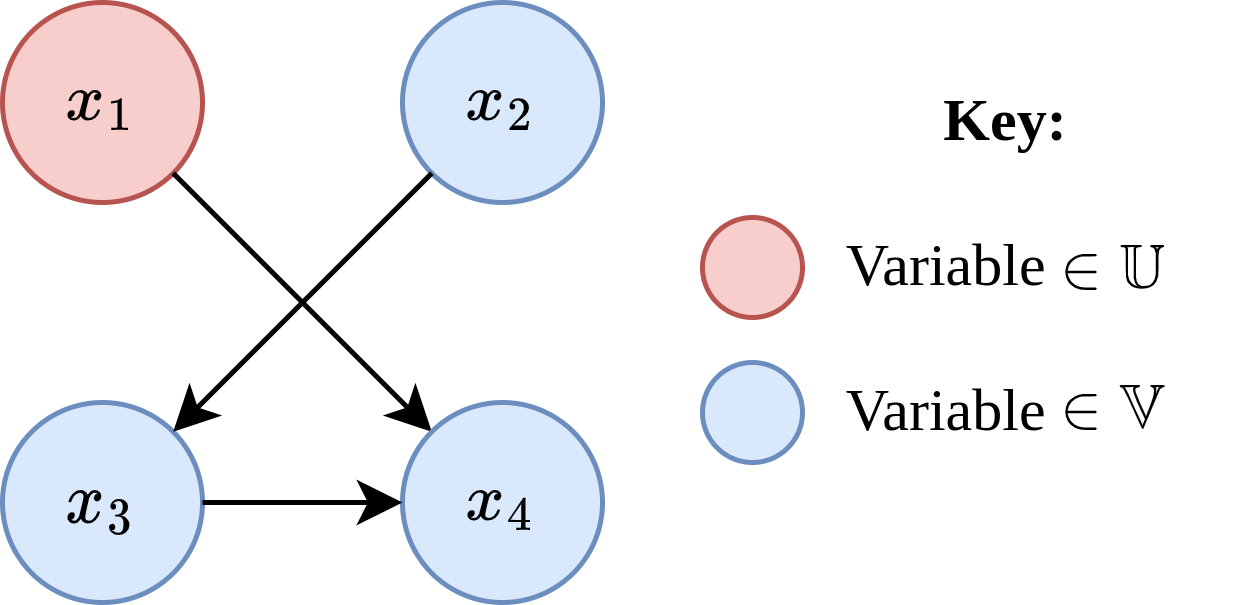
\includegraphics[width=0.25\linewidth]{images/draw.io/Simple SCM Severed.png}
	\caption{Causal graph $\mathcal{G}$ of SCM $\mathcal{M}_1$.}
	\label{fig:toy_scm_severed}
\end{figure}

\begin{align}
	x_1 & = u_1 \\ \nonumber
	x_2 & = 30,000 \\ \nonumber
	x_3 & = u_3 - 0.25x_2 \\ \nonumber %debt
	x_4 & = \frac{x_3}{x_1} %debt to income ratio
\end{align}

\textbf{3. Prediction}. Using the updated model $\mathcal{M}_1$ and values of exogenous variables $\mathbf{u}$, calculate the values of the endogenous variables.

\begin{align}
	x^{\text{SCF}}_1 & = u_1 &  = 30,000 \\ \nonumber
	x^{\text{SCF}}_2 & = 30,000 & = 30,000 \\ \nonumber
	x^{\text{SCF}}_3 & = u_3 - 0.25x^{\text{SCF}}_2 = 16,250 - 0.25(30,000) & = 8,750 \\ \nonumber
	x^{\text{SCF}}_4 & = \frac{x^{\text{SCF}}_3}{x^{\text{SCF}}_1} = \frac{8,750}{30,000} & = 0.292
\end{align}

Mathematically, we can denote the Action-Abduction-Prediction steps as shown in equation \ref{eq:hard_intervention}, where $I$ is the set of indices of intervened on variables, $\delta_i$ is the action on variable $i$, $f_i \in \mathbb{F}$ is structural equation of the variable $i$,  $\text{pa}_i$ are the parents of variable $i$, $I$ is the set of variables that intervened upon (e.g, ) and $\mathbb{I}$ is the indicator function.

\begin{align} \label{eq:hard_intervention}
	x^{\text{SCF}}_i = & \mathbb{I}_{i \in I} (x_i + \delta_i) + \mathbb{I}_{i \notin I} \bigg(x_i + f_i(\text{pa}^{\text{SCF}}_i) - f_i(\text{pa}_i)\bigg)
\end{align}


To calculate recourse $\mathbf{x}^*$ with an SCM over all the features within $\mathbf{x}$, we need to re-formulate the original algorithmic recourse optimisation problem presented in equation \ref{eq:recourse_setup}. Following \textcite{karimiAlgorithmicRecourseCounterfactual2021}, we replace the minimising the cost of changing features from $\mathbf{x}$ to $\mathbf{x}'$ with minimising the cost of \textit{interventions} $A = \text{do} \{\mathbf{x}_i:=\mathbf{x}_i + \boldsymbol{\delta}_i\}_{i=1, \ldots, D}$ where $D$ is the number of features. The updated recourse problem is shown in equation \ref{eq:causal_recourse_problem_hard}.

\begin{align} \label{eq:causal_recourse_problem_hard}
	A^* = & \argmin_{A} \texttt{cost}(\mathbf{x}, A) \\ \nonumber
	\text{s.t. } & h(\mathbf{x}^{\text{SCF}}) = 1, \\ \nonumber
	& \mathbf{x}^{\text{SCF}}_i = \mathbb{I}_{i \in I} (\mathbf{x}_i + \boldsymbol{\delta}_i) + \mathbb{I}_{i \notin I} \bigg(x_i + f_i(\textbf{pa}^{\text{SCF}}_i) - f_i(\textbf{pa}_i)\bigg), \\ \nonumber
	& A \in \mathcal{F}
\end{align}

We define the cost of interventions $A$ on original features $\mathbf{x}$ as the sum of the cost of the individual actions. The cost of each individual action is left to be flexible, and can represent a variety of cost functions, such as the $L_p$-norm of $\boldsymbol{\delta}_i$ or a percentile shift based cost function such as that used by \textcite{ustunActionableRecourseLinear2019}.

\begin{equation}
	\texttt{cost}(\mathbf{x}, A) = \sum_{i=1}^{D} c \bigg(\text{do}(\mathbf{x}_i:=\mathbf{x}_i + \boldsymbol{\delta}_i) \bigg)
\end{equation}

This formulation relies on two key assumptions.

\textbf{Assumption 1}. The interventions are structural (hard) interventions, where after intervening on a variable, all incoming edges to its corresponding node in the causal graph are severed. If an individual were to intervene on savings ($x_2$) (perhaps by selling their car or borrowing from family), then we assume that they then stop saving a proportion of their income (severing the edge between $x_1$ and $x_2$).

\textbf{Assumption 2}. Interventions on multiple variables are carried out simultaneously. Given an intervention A = [£32,000, £27,500, £10,000, 1/3]$^T$, it is assumed that salary as increased at the same time as savings, as opposed to taking place sequentially.

\subsection{Soft (Parametric) Interventions} \label{section:soft_interventions}

In many cases where recourse is provided, such as credit scoring, it is unlikely that intervening on a variable leads to all incoming edges to its corresponding node in the causal graph being severed - a violation of assumption 1. Intervening on savings is unlikely to lead to an individual stopping saving their salary. Likewise, intervening on body fat levels through liposuction does not lead to diet having no causal effect on body fat levels. Structural (hard) interventions are typically used in randomised control trials. For example, in a medical trial, patients are assigned to either to receive either a treatment or a placebo. Any other variables that may have caused the patient to receive a treatment or not now have no causal effect, as in carrying out the trial we simply assign the patient to receive either the treatment or a placebo.

In the cases where assumption 1 is violated, we can then represent the interventions as soft (or parametric) interventions, which do not result in severing of incoming edges \citep{eberhardtInterventionsCausalInference2007}. After the soft (parametric) intervention, we denote the resulting value of $\mathbf{x}$ after the intervention as $\mathbf{x}^{\text{PCF}}$, the \textit{parametric} counterfactual, which is defined below.

\begin{equation} \label{eq:soft_interventions}
	x^{\text{PCF}}_i = \mathbb{I}_{i \in I} \delta_i + \bigg( x_i + f_i(\text{pa}^{\text{PCF}}_i) - f_i(\text{pa}_i) \bigg)
\end{equation}

As the majority of interventions which take place in the context of algorithmic recourse, such as increasing savings and re-taking an test such as the GMAT/GRE (in the case of recourse for postgraduate admissions) do not tend to result in the severing of incoming edges such as the proportion of income saved and the effect of additional revision on test scores, soft interventions are implemented in this thesis. Using soft interventions results in an updated causal recourse problem shown below in equation \ref{eq:causal_recourse_problem_soft}.

\begin{align} \label{eq:causal_recourse_problem_soft}
	A^* = & \argmin_{A} \texttt{cost}(\mathbf{x}, A) \\ \nonumber
	\text{s.t. } & h(\mathbf{x}^{\text{PCF}}) = 1, \\ \nonumber
	& 	\mathbf{x}^{\text{PCF}} = \mathbb{I}_{i \in I} \boldsymbol{\delta}_i + \bigg( \mathbf{x}_i + f_i(\textbf{pa}^{\text{PCF}}_i) - f_i(\textbf{pa}_i) \bigg), \\ \nonumber
	& A \in \mathcal{F}
\end{align} 


\subsection{Sequential Interventions}

Assumption 2 of the causal recourse problem formulation in \ref{eq:hard_intervention} is that all interventions occur simultaneously. Picture a scenario where an individual is rejected from a PhD program, and the recourse interventions are to gain more research experience (potentially through a pre-doctoral fellowship or research assistant position) and obtain a more favourable letter of recommendation. In the real world, it is likely that these actions will be carried out sequentially, where research experience is obtained first and the letter of recommendation is second (as the professor for whom the applicant is conducting their research under will likely be the author of the letter of recommendation), as opposed to occurring simultaneously.

Using equation \ref{eq:soft_interventions}, the order of the intervention does not affect the counterfactual values\comment{Potentially worth showing how $f_i(\text{pa}^{\text{PCF}}_i)$ in one intervention is cancelled out by $f_i(\text{pa}_i)$ in the next intervention} $x^{\text{PCF}}_i$, but can affect the cost of actions $A$.


\begin{proposition} \label{sequential_proposition}
	In a sequential intervention setting with $n$ separate interventions where $x_i$ and $x_j$ are intervened upon, if the cost of individual interventions $c(\text{do}(x_i:=x_i + \delta_i))$ depends on the value of $x_i$ and $x_i$ is a descendent of $x_j$, then the ordering of the sequential interventions affects the total cost of the $n$ sequential interventions.
\end{proposition}

\begin{proof}
	The values of $x_i$ after an intervention on $x_i$ and intervening on $x_j$ are shown below.
	\begin{align} \label{eq:proposition_1_equation}
		x^{\text{PCF}_i}_i & = x_i + \delta_i \\ \label{eq:proposition_1_equation2}
		x^{\text{PCF}_j}_i & = x_i + f_i(\text{pa}^{\text{PCF}}_i) - f_i(\text{pa}_i)
	\end{align}
	As the cost of individual interventions depends on the value of $x_i$ before intervention, the cost of intervening on $x_i$ first depends on the value $x_i$ whereas the cost of intervening on $x_i$ second depends on the value $x_i + f_i(\text{pa}^{\text{PCF}}_i) - f_i(\text{pa}_i)$ (the value after intervening on $x_j$, seen in equation \ref{eq:proposition_1_equation2}). This results in different costs for the intervention on $x_i$ for the different orderings.
	
	As $x_j$ is a descendant of $x_i$, the intervention on $x_i$ has no effect on $x^{\text{PCF}_i}_j$ and both intervening on $x_j$ first or second leads to the same cost for the intervention on $x_j$.
	
	As the total cost is the sum of the costs of each intervention and the costs for the interventions on $x_i$ are different for each ordering and the intervention on $x_j$ are the same for each ordering, then the total cost for the two orderings of sequential interventions are different. \comment{Make this more maths-y and potentially add a worked example}
\end{proof}

To take into account the potential effects of different orderings on the costs, we denote interventions as an ordered set $A = \big\{(\mathbf{S}, \text{do} \{\mathbf{x}_i:=\mathbf{x}_i + \boldsymbol{\delta}_i\}_{i=1, \ldots, D})\big\}$ where $\mathbf{S}$ is a permutation of the set $\{1, \ldots, D\}^N$ and represents the ordering of the intervention.\comment{To replace $o_i$ with a permutation set?} Given this updated definition of $A$, the causal recourse formulation stays the same as shown in \ref{eq:causal_recourse_problem_soft}.

\section{Differentiable Sorting}

In order to solve equation \ref{eq:causal_recourse_problem_soft} with sequential interventions, we need to optimise for an ordering of interventions.\comment{Is this NP-hard?} With $D$ features, there are $D!$ different orderings (i.e. permutations of the set $\{1, \ldots, D\}$) and equation \ref{eq:causal_recourse_problem_soft} becomes a combinatorial optimisation problem.\comment{I think this is true, to check}

In order to transform the combinatorial optimisation problem to a continuous optimisation problem, we can first define a vector $O\in \mathbb{R}^{D}$, which can be optimised using continuous heuristics such as gradient descent. From $O$, we can recover $S$ through the transformation $S = \argsort(O)$, where $\argsort(O)$ returns the indexes of $O$ that sorts $O$ in ascending order. By optimising for $O$, we indirectly optimise the ordering $S$ as $S$ is defined as $S = \argsort(O)$.

However, the operation $\argsort$ (a piecewise-constant function) is not differentiable. As a solution, we replace the $\argsort$ operator with the $\softsort$ operator, a continuous relaxation of the $\argsort$ operator \citep{prilloSoftSortContinuousRelaxation2020}.

For a given permutation (i.e., ordering) $\pi \in \{1, \ldots, D\}^D$, we can also express the permutation $\pi$ as a permutation matrix $P_{\pi} \in \{0,1\}^{D \times D}$. We can represent $P_{\pi}$ mathematically as a square matrix with values as shown in equation \ref{eq:permutation_matrix_def}. For example, the permutation matrix of the permutation $\pi = [3, 1, 2]^T$ is shown in equation \ref{eq:permutation_matrix_example}. 

\begin{equation} \label{eq:permutation_matrix_def}
	P_{\pi}[i,j] = \begin{cases}
		1 & \text{ if } j = \pi_i \\
		0 & \text{ otherwise}
	\end{cases}
\end{equation}

\begin{align} \label{eq:permutation_matrix_example}
	\pi = [3, 1, 2]^T \Longrightarrow	P_{\pi} = 
	\left[\begin{array}{lllll}
		0 & 0 & 1 \\
		1 & 0 & 0 \\
		0 & 1 & 0
	\end{array}\right]
\end{align}

$\softsort$ defines a continuous relaxation for $P_{\argsort(O)}$, defined in equation \ref{eq:softsort_def}, where $d$ is a differentiable (almost everywhere) semi-metric function and $\tau >0$ is a temperature parameter that controls the degree of approximation. For the experiments in this thesis, $d(x,y) = |x-y|$ has been used.

\begin{equation} \label{eq:softsort_def}
	\texttt{SoftSort}^d_{\tau}(O) = \texttt{softmax}\bigg( \frac{-d(\texttt{sort}(O)\mathbbm{1}^T, \mathbbm{1}O^T)}{\tau} \bigg)
\end{equation}

The value of the semi-metric function $d$ is larger when $\texttt{sort}(O)[i]$ is close to $O[j]$ and smaller when $\texttt{sort}(O)[i]$ is far from $O[j]$. The $\texttt{softmax}$ function is applied row-wise, meaning that the larger the value of semi-metric function $d$ compared to other values, the larger the value of $\texttt{SoftSort}[i,j]$. A larger temperature parameter $\tau>0$ leads to the values of $d$ moving closer together and, after the $\texttt{softmax}$, the values of $\texttt{SoftSort}[i,j]$ become more evenly distributed, compared to the true $P_{\argsort(O)}$, which is binary (i.e., very unevenly distributed). Therefore, the larger the value of $\tau$, the more approximate $\softsort$ becomes. As $\tau \to 0$, $\softsort^d_{\tau}(O) \to P_{\argsort(O)}$.

A visual representation can be seen below of $P_{\argsort(O)}$ and $\texttt{SoftSort}^{|\cdot|}_{1}(O)$ can be seen below for $O = [2,5,4]^T$.

\begin{equation}
	O = \begin{bmatrix}
		2 \\
		5 \\
		4
	\end{bmatrix}
	\Longrightarrow
	P_{\argsort(O)} =
	\begin{bmatrix}
		0 & 1 & 0 \\
		0 & 0 & 1 \\
		1 & 0 & 0 \\
	\end{bmatrix}
\end{equation}

\begin{equation} \label{eq:softsort_example}
	\texttt{SoftSort}^{|\cdot|}_{1}(O) = 
	\texttt{softmax} \Bigg(-\begin{bmatrix}
		|5-2| & |5-5| & |5-4| \\
		|4-2| & |4-5| & |4-4| \\
		|2-2| & |2-5| & |2-4|
	\end{bmatrix} \Bigg)	
	=
	\begin{bmatrix}
		0.04 & \textbf{0.70} & 0.26 \\
		0.09 & 0.24 & \textbf{0.67} \\
		\textbf{0.85} & 0.04 & 0.11
	\end{bmatrix}
\end{equation}

As $\softsort$ is the combination of the $\texttt{softmax}$ function (which is differentiable), the semi-metric $d$ (which is differentiable almost everywhere) and the $\texttt{sort}$ function (which is differentiable almost everywhere), this leads to $\softsort$ being differentiable (almost everywhere).

The values of the matrix that $\softsort$ produces, such as in equation \ref{eq:softsort_example}, can be interpreted \textit{loosely} as the probability that the $i^{\text{th}}$ element of $\pi_{\argsort(O)}$ is $j$.

When incorporating $\softsort$ into the the causal recourse problem defined in equation \ref{eq:causal_recourse_problem_soft}, we take the maximum `probability' in each row as the ordering $S$, as opposed to weighting the costs of differing orderings by their `probabilities'.

\section{Generating Recourse} \label{section:generating_recourse}

To generate recourse, we need to solve the below constrained optimisation problem from equation \ref{eq:causal_recourse_problem_soft}, where $A$ is the ordered set $A = \big\{(\mathbf{S}, \text{do} \{\mathbf{x}_i:=\mathbf{x}_i + \boldsymbol{\delta}_i\}_{i=1, \ldots, D})\big\}$.

\begin{align}
	A^* = & \argmin_{A} \texttt{cost}(\mathbf{x}, A) \\ \nonumber
	\text{s.t. } & h(\mathbf{x}^{\text{PCF}}) = 1, \\ \nonumber
	& 	\mathbf{x}^{\text{PCF}} = \mathbb{I}_{i \in I} \boldsymbol{\delta}_i + \bigg( \mathbf{x}_i + f_i(\textbf{pa}^{\text{PCF}}_i) - f_i(\textbf{pa}_i) \bigg), \\ \nonumber
	& A \in \mathcal{F}
\end{align} 

To solve this problem, we convert the problem from a constrained optimisation problem to a unconstrained optimisation problem and solve using gradient descent. We make use of Lagrange multipliers to reach the problem formulation as a min-max objective with constraint that the classifier scores the updated feature values $\mathbf{x}^{\text{PCF}}$ with a score of at least 0.5 (this can be changed for a given classifier score).

\begin{equation} \label{eq:lagrange}
	\min_{A \in \mathcal{F}} \max_{\boldsymbol{\lambda}} \sum_{i=1}^D \texttt{cost}(\mathbf{x}, A) - \boldsymbol{\lambda} \bigg( h(\mathbf{x}^{\text{PCF}}) - 0.5\bigg)
\end{equation}

This expression is then optimised using gradient descent where in each epoch, a gradient descent step is taken for $\boldsymbol{\lambda}$ and then another gradient step is taken for $A$. The expression is optimised until $h(\mathbf{x}^{\text{SCF}})$ converges to 0.5.\\

Once the optimisation has converged, we are left with optimal actions $A^*$ for a given classifier $h$, cost function $\cost$ and structural causal model $\mathcal{M}$. From the optimal actions, we can obtain the structural counterfactual feature values $\mathbf{x}^{\text{PCF}}$. It is these feature values that are presented to the negatively classified individuals, as opposed to the actions themselves.\\

We only present $\mathbf{x}^{\text{PCF}}$ because, whilst we know that $h(\mathbf{x}^{\text{PCF}})=1$, we cannot guarantee that $h(\mathbf{x}^{\text{PCF}})=1$ 
unless there is perfect knowledge of the structural causal model. To demonstrate this, we will re-use the SCM from equation \ref{eq:toy_structural_equations}, which we denote as $\mathcal{M}^{\text{TRUE}}$.

\begin{align}
	x_1 & = u_1 & u_1 \sim N(30 , 5) \\ \nonumber %income
	x_2 & = u_2 + 0.5x_1 & u_2 \sim N(20, 10) \\ \nonumber %savings
	x_3 & = u_3 - 0.25x_2 & u_3 \sim \text{Uniform}(0, 20) \\ \nonumber %debt
	x_4 & = \frac{x_3}{x_1} %debt to income ratio
\end{align}

Suppose the true SCM was misspecified and we instead used $\mathcal{M}^{\text{FALSE}}$, which is the same as $\mathcal{M}^{\text{TRUE}}$, with the exception of the relationship between $x_1$ and $x_2$ (income and savings). In $\mathcal{M}^{\text{FALSE}}$, the relationship is shown below.

\begin{equation}
	x_2 = u_2 + x_1
\end{equation}

For an individual with original features [30, 25, 10, 1/3]$^T$, where $h$ is a linear classifier with bias $b=0$ and weights $w=[0.2, 0.2, -1.25, -3]$, they are initially negatively classified (8\% of approval). Using $\mathcal{M}^{\text{FALSE}}$, they are provided actions $\text{do}(\mathbf{x}_1=35)$, which results in $\mathbf{x}^{\text{SCF}} = [35, 30, 8.75, 0.25]^T$ and would result in a positive classification (79\% chance of approval). However, as $\mathcal{M}^{\text{FALSE}}$ is a misspecified SCM, the true structural counterfactual from $\text{do}(\mathbf{x}_1=35)$ is $\mathbf{x}^{\text{SCF}} = [35, 27.5, 9.375, 0.27]^T$, which results in a negative classification (49\% chance of approval). \textcite{karimiAlgorithmicRecourseImperfect2020} provide a more formal proof that, that if the true SCM is not known, then recourse cannot be guaranteed when only providing interventions. \comment{expand this explanation, is a bit too dense}












% Cost Learning
\chapter{Cost Learning}


\section{Learning from revealed preferences}

We do not observe the cost function itself, but one way to approximate it is to \textit{learn from revealed preferences} (see section \ref{section:revealed_pref_lit}). We propose that each individual who is negatively classified is presented with $N$ pairs of recourse options $((\mathbf{a}_n^1, \mathbf{o}_n^1),(\mathbf{a}_n^2, \mathbf{o}_n^2))$. Each of the recourse options corresponds to a list of actions and associated orderings. The individuals, for each of the $N$ pairs of recourse options, then select which one is preferable. \comment{Need to rephrase actions as the total action (even if you get part of it for 'free'.}

If, for a single pair of recourse options $((\mathbf{a}_n^1, \mathbf{o}_n^1),(\mathbf{a}_n^2, \mathbf{o}_n^2))$, option 1 is selected, then we assume that $\sum_{i=1}^D c(\mathbf{a}^1_{ni}) \leq \sum_{i=1}^D c(\mathbf{a}^2_{ni})$. If option 2 is selected, we assume the opposite, that $\sum_{i=1}^D c(\mathbf{a}^1_{ni}) > \sum_{i=1}^D c(\mathbf{a}^2_{ni})$. The responses to the pairs of recourse options presented (the pairwise comparisons) reveal information about the individuals' preferences over recourse options, i.e., their cost functions over individual features. \comment{User preference over cost functions involves knowledge of the causal graph, should this then be optimised for in learning from revealed preferences.)}

Once a cost function is learned, we need to solve the optimisation problem mentioned in equation \ref{eq:lagrange_formulation} to generate the recourse $(\mathbf{a}', \mathbf{o}')$.

\subsection{Weighted Squared Costs}

Let the individual cost function take the form $c(\mathbf{a}, \beta) = \sum_{i=1}^D \beta_i \mathbf{a}^2_i$, where $\beta \in \mathbb{R}^D$ is a vector which expresses the mutability of each feature $i$. To learn the cost function, we need to learn $\beta$.

Given a fixed weighted adjacency matrix $W$,\comment{Seems much more efficient to assume a fixed ordering} we can denote the response of the $n$th paired comparison as follows.

\begin{equation} \label{eq:paired_response}
	y_{n} = \begin{cases}
		-1 & \text{if } \sum_{i=1}^D c(\mathbf{a}^1_{ni}) \leq \sum_{i=1}^D c(\mathbf{a}^2_{ni}) \\
		+1 & \text{if }  \sum_{i=1}^D c(\mathbf{a}^1_{ni}) > \sum_{i=1}^D c(\mathbf{a}^2_{ni}) \\
	\end{cases}
\end{equation}

We optimise for when $y_n$ and $\hat{y}_n$ (the predicted value of $y_n$, using our initial guess of $\beta$) are similar. A optimisation to do this is shown below, where there are $K$ individuals and $N$ pairwise comparisons and $\ell(y, \hat{y}) = \max[0, 1-y\hat{y}]$ represents the hinge loss.

\begin{equation}
	\argmin_\beta = \frac{1}{KN} \sum_{k=1}^K \sum_{n=1}^N \ell (y_{kn}, \hat{y}_{kn}(\beta)) + \underbrace{\lambda ||\beta||_2}_{\text{L2 regularisation}}
\end{equation}

This is an unconstrained optimised problem that can be optimised via gradient descent. However, operation in equation \ref{eq:paired_response} is non, differentiable, so instead it is approximated with the below expression, which fits $\hat{y}_n$ into [-1,1] where $\lambda$ is a hyperparameter regularising for 'confidence' of the predictions.

\begin{equation}
	\hat{y}_n = \tanh \Bigg(\lambda \Big(\sum_{i=1}^D c(\mathbf{a}^1_{ni}) - \sum_{i=1}^D c(\mathbf{a}^2_{ni})\Big)\Bigg)
\end{equation}


\section{Mahalanobis distance}

The Mahalanobis distance between the vector $\mathbf{x}$ and the vector $\mathbf{y}$ is defined in equation \ref{eq:mahalanbobis_distance}, where $M$ is a positive semi-definite matrix.

\begin{equation} \label{eq:mahalanbobis_distance}
	||\mathbf{x-y}||_{\mathbf{M}} = \sqrt{(\mathbf{x-y})^T\mathbf{M}^{-1}(\mathbf{x-y})}
\end{equation}

The matrix $\mathbf{M}$ captures different relationships between the features within $\mathbf{x}$ and $\mathbf{y}$ in the off-diagonal elements of $\mathbf{M}$. If $\mathbf{M}$ is set to the identity matrix, then the Mahalanobis distance then becomes equal to the Euclidean distance between $\mathbf{x}$ and $\mathbf{y}$. \\

\subsection{Learning the Mahalanobis distance}

In order to use the Mahalanobis distance as a cost function, we must learn the matrix $\mathbf{M}$. In this set-up, each individual $k$ with original features $\mathbf{x}_k$ is presented with $N$ recourse options $(\mathbf{x}_{kn}^a, \mathbf{x}_{kn}^b)$. The response $y_{kn}$ is defined in equation \ref{eq:response_definition}, where $c^G_k$ represents the ground truth cost function of individual $k$.

\begin{equation} \label{eq:response_definition}
	y_{kn} = \begin{cases}
		-1 & \text{if } c^G_k(\mathbf{x}_{kn}, \mathbf{x}^a_{kn}) \leq c^G_k(\mathbf{x}_{kn}, \mathbf{x}^b_{kn}) \\
		+1 & \text{if } c^G_k(\mathbf{x}_{kn}, \mathbf{x}^a_{kn}) > c^G_k(\mathbf{x}_{kn}, \mathbf{x}^b_{kn}) \\
	\end{cases}
\end{equation}

To optimise for $\textbf{M}$, we compare the squared Mahalanobis distances between $\textbf{x}_k$ and $\textbf{x}^a_{kn}$ and between $\textbf{x}_k$ and $\textbf{x}^b_{kn}$. The optimisation problem to learn $\textbf{M}$ is shown in equation \ref{eq:mahalanobis_non_convex}, where $\ell$ represents either the hinge or logistic loss function. The optimisation is an adaptation of the optimisation problem presented in \textcite{canalOneAllSimultaneous2022}.

[\textbf{TO ADD EXPLANATION ON WHY THIS IS A GOOD OPTIMISATION}]

\begin{align} \label{eq:mahalanobis_non_convex}
	\min_{\mathbf{M}} & \frac{1}{KN} \sum_{k=1}^K \sum_{n=1}^N \ell \bigg( y_{kn} \big(|| \mathbf{x}_k - \mathbf{x}_{kn}^a ||^2_{\mathbf{M}} - || \mathbf{x}_k - \mathbf{x}_{kn}^b ||^2_{\mathbf{M}} \big) \bigg) \\	
	\text{s.t. } & \mathbf{M} \succeq 0, \nonumber
\end{align}

\section{Convex layers}

To look into convex neural networks using \href{https://github.com/cvxgrp/cvxpylayers}{\texttt{cvxpylayers}}, which is based on \textcite{agrawalDifferentiableConvexOptimization2019}.


% Experiments
\chapter{Experiments} \label{chapter:experiments}

In this chapter, we evaluate how effective our learned cost function is, which is described below, where $D$ is the number of features, $A$ is the set of actions and the resulting value of $\mathbf{x}$ after the interventions is $\mathbf{x}^{\text{PCF}}$.

\begin{align} \label{eq:cost_function_experiments}
	\cost(A, \beta_k, \mathcal{F}) & = \sum_{i=1}^D \delta_i \beta_{ki}^2 \\ \nonumber
	A & = \big\{(\mathbf{S}, \text{do} \{\mathbf{x}_i:=\mathbf{x}_i + \boldsymbol{\delta}_i\}_{i=1, \ldots, D})\big\} \\ \nonumber
	\mathbf{x}^{\text{PCF}} & = \mathbb{I}_{i \in I} \boldsymbol{\delta}_i + \bigg( \mathbf{x}_i + f_i(\textbf{pa}^{\text{PCF}}_i) - f_i(\textbf{pa}_i) \bigg)
\end{align}

\section{End-to-End Methodology}

The end to end methodology for generating recourse with a learned cost is shown in Figure \ref{fig:workflow}, and more details on each of the steps in the methodology are described below.

\begin{figure}[!htb]
	\centering
	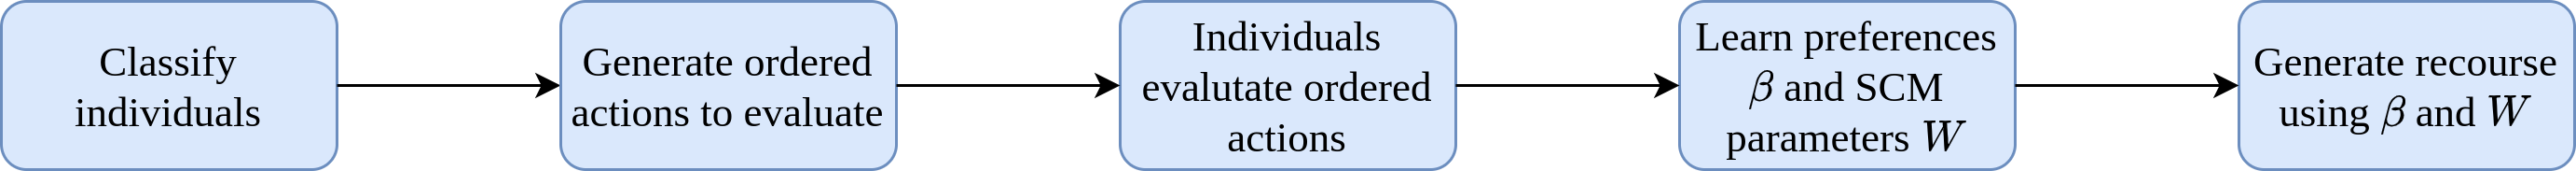
\includegraphics[width=\linewidth]{images/draw.io/workflow.png}
	\caption{End-to-End Methodology}
	\label{fig:workflow}
\end{figure}

\begin{enumerate}
	\item \textbf{Classify individuals}. Individuals with features $\mathbf{X}$ are assessed by a classifier and are classified either positively (e.g., loan approved, admission acceptance) or negatively (e.g., loan rejected, admission rejected). In this thesis, logistic regression has been used, largely for simplicity. However, as an augmented Lagrangian gradient descent optimisation is used to generate recourse (see section \ref{section:generating_recourse}), any differentiable classifier could be used instead of logistic regression.
	
	\item \textbf{Generate ordered actions to evaluate}. We randomly generate actions for each negatively classified individual and associated randomly generated orderings. This is another area for future work, where an online or Bayesian approach could be used to generate recourse actions in order to maximise information gain, such as the approach used in \textcite{detoniPersonalizedAlgorithmicRecourse2023}.
	
	\item \textbf{Users evaluate ordered actions}. Using the cost function described in equation \ref{eq:cost_function_experiments} with noisy user preferences $\tilde{\beta_k}$ and noisy SCM $\tilde{\mathcal{F}}$, users evaluate which of the ordered actions they are presented with they prefer. 
	
	\item \textbf{Learn preferences $\hat{\beta_k}$ and SCM approximation parameters $\hat{W}$}. The model deployer then learns user preferences $\hat{\beta_k}$ and a linear approximation of the true SCM $\hat{W}$ using the optimisation presented in section \ref{section:cost_learning_formulation}.
	
	\item \textbf{Generate recourse using $\hat{\beta_k}$ and $\hat{W}$}. The model deployer then generates recourse $\mathbf{X}^*$ for the negatively classified users.
	
\end{enumerate}



\section{Synthetic Data}

We create synthetic SCMs, from which we sample our data $\mathbf{X}$. We simulate two different SCMs, the first being a linear SCM and the second a non-linear SCM. In both cases, we assign individuals to have the same randomly generated feature mutability $\beta$ plus some noise. This means that individuals tend to have similar preferences, but do not have the same preferences.

\subsection{Linear SCM} \label{section:linear_scm}

Shown below are the structural equations of the linear SCM $\mathcal{M}_{\text{LIN}}$ as well as the associated causal graph.

\begin{align}
	x_1 & = u_1 & u_1 \sim N(0,1) \\ \nonumber
	x_2 & = u_2 + 0.5x_1 & u_2 \sim N(0,1) \\ \nonumber
	x_3 & = u_3 + 0.2x_1 + 0.3x_2 & u_3 \sim N(0,0.5) \\ \nonumber
	y   & \sim \text{Bernoulli}(\sigma(0.1x_1 + 0.2x_2 + 0.3x_3))
\end{align}

\begin{figure}[!htb]
	\centering
	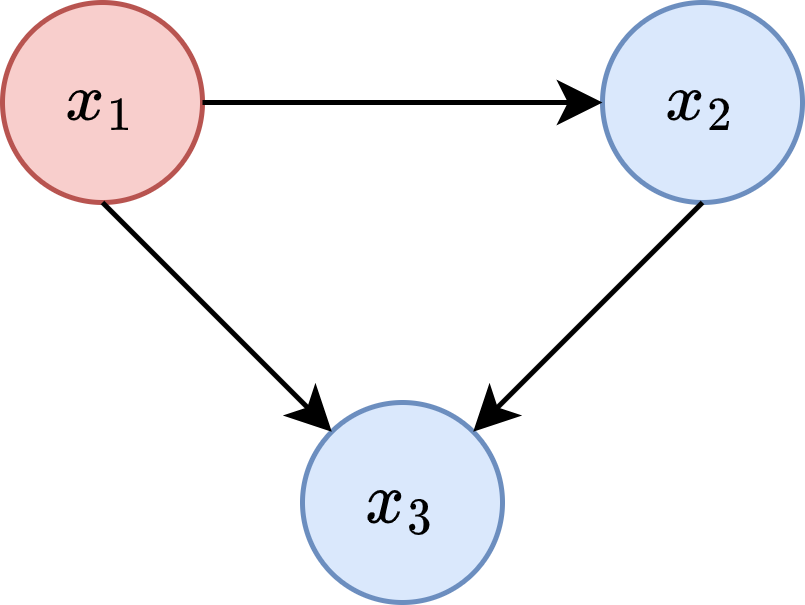
\includegraphics[width=0.4\linewidth]{images/draw.io/toy_scm.png}
	\caption{Linear SCM $\mathcal{M}_{\text{LIN}}$}
	\label{fig:simple_scm}
\end{figure}

\subsection{Non-Linear SCM}

Shown below are the structural equations of the non-linear SCM $\mathcal{M}_{\text{NL}}$ as well as the associated causal graph.

\begin{align}
	x_1 & = u_1 & u_1 \sim N(0,1) \\ \nonumber
	x_2 & = u_2 - \frac{2}{1 + x_1^2} & u_2 \sim N(0,1) \\ \nonumber
	x_3 & = u_3 + 0.2x_1 + 0.1x_1x_2 & u_3 \sim N(0,0.5) \\ \nonumber
	x_4 & = u_4 + 0.4x_1 + 0.7x_2x_3 & u_4 \sim N(0,0,5) \\ \nonumber
	x_5 & = u_5 + 0.8x_1 & u_5 \sim N(0,0.5) \\ \nonumber
	y   & \sim \text{Bernoulli}(\sigma(0.1x_1 + 0.2x_2 + 0.3x_3 + 0.4x_4 + 0.5x_5))
\end{align}

\begin{figure}[!htb]
	\centering
	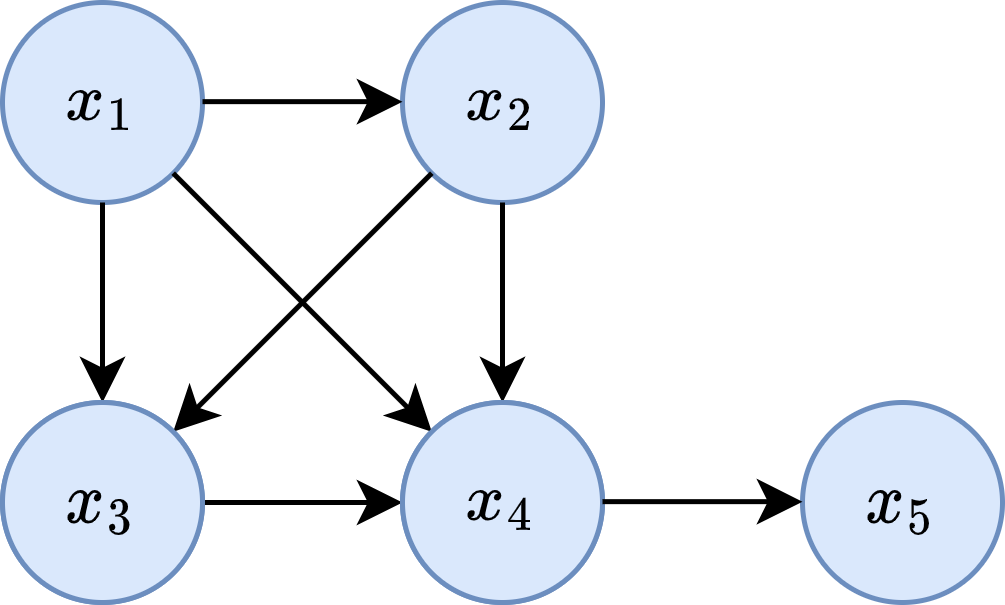
\includegraphics[width=0.5\linewidth]{images/draw.io/non_linear_scm.png}
	\caption{Non-Linear SCM $\mathcal{M}_{\text{NL}}$}
	\label{fig:non_linear_scm}
\end{figure}


\section{Evaluation Criteria} \comment{can probably ditch this section, consider have basically got rid of it}

To how useful the learned user preferences $\hat{\beta_k}$ and SCM approximation parameters $\hat{W}$ are, we need to be able to evaluate $\cost(\mathbf{x,x}^*)$, where $\mathbf{x}^*$ represents the recourse generated. To do this, we propose simply minimise the squared distance between the recourse $\mathbf{x}^*$ and $\mathbf{x}'$, which represents the parametric counterfactual from ordered actions $A$ under the true SCM. The objective function that is optimised is shown below.

\begin{equation}
	A^* = \argmin_{A} (\mathbf{x}^* - \mathbf{x}')^2
\end{equation}

where

\begin{align}
	A & = \big\{(\mathbf{S}, \text{do} \{\mathbf{x}'_i:=\mathbf{x}'_i + \boldsymbol{\delta}_i\}_{i=1, \ldots, D})\big\} \\ \nonumber
	{\mathbf{x}'}^{\text{PCF}} & = \mathbb{I}_{i \in I} \boldsymbol{\delta}_i + \bigg( \mathbf{x}'_i + f_i(\textbf{pa}^{\text{PCF}}_i) - f_i(\textbf{pa}_i) \bigg)
\end{align}

This can be optimised using gradient descent. Once we have obtained ordered actions $A^*$ that lead to our recourse $\mathbf{x}^*$ under the true SCM, we can calculate $\cost(\mathbf{x,x}')$ as $\cost(A^*, \beta_k, \mathcal{F})$ as defined in equation $\ref{eq:cost_function_experiments}$, where $\beta_k$ represents the true user preferences and $\mathcal{F}$ are the true structural equations.

\section{Results}

In this section, we present the results of the learned cost function on the two SCMs described in the previous section. In all the experiments conducted in this section, we simulate 2,000 individuals from the SCMs, which are then classified either positively or negatively.

\subsection{Linear SCM}

In this section, we detail the performance of our methodology on the linear SCM outlined in section \ref{section:linear_scm}. We compare the cost of the recourse we generated to the cost of the recourse generated using the ground truth user preferences $\beta_k$ and the ground truth SCM. Assuming that there is no noise in either the users' evaluation of their own preferences and their local evaluation of the SCM, we have calculated the percentage increase in cost of the recourse generated compared to the ground truth recourse.

\begin{table}[!htb]
	\centering
	\begin{tabular}{l|l|l}
		\hline
		\textbf{Model} & \textbf{Cost} & \textbf{Increase in cost (\%)} \\
		\hline
		Ground truth   & 0.214 & 0\%                        \\
		Identity $W$   & 0.363 & 69.5\%                     \\
		5 comparisons  & 0.332 &  55.1\%                     \\
		10 comparisons & 0.290 &  35.4\%                     \\
		20 comparisons & 0.250 &  16.7\%                     \\ 
		50 comparisons & 0.224 &  4.6\%                      \\ \hline
	\end{tabular}
	\caption{Ground truth cost of recourse }
\end{table}


\subsection{Non-Linear SCM}



================================================

[TO CLEAN UP]

\begin{figure}[!htb]
	\centering
	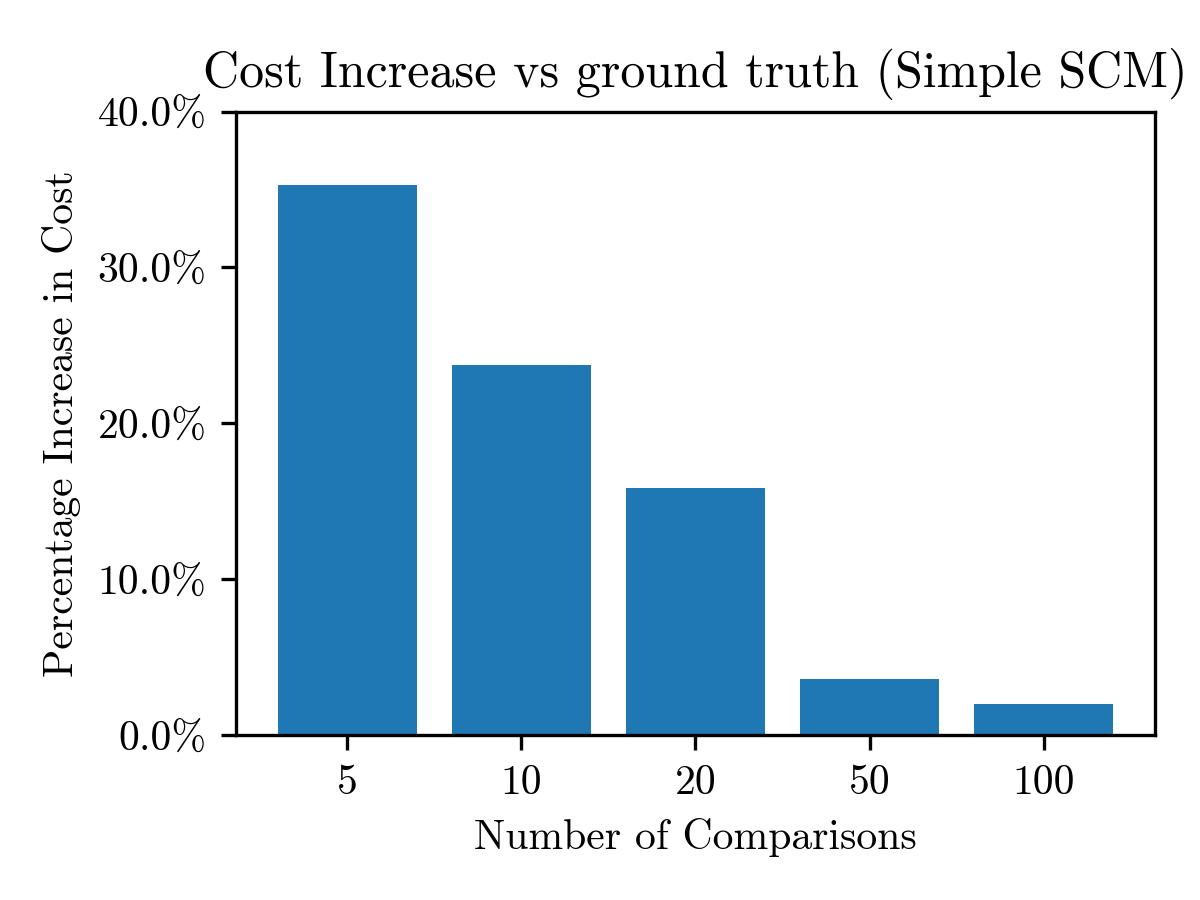
\includegraphics[scale=1]{images/simpleSCM_comparison_results.png}
	\caption{Comparison of the average cost of recourse for learned costs functions compared to the ground truth cost function for the Simple SCM.}
	\label{fig:simple_scm}
\end{figure}


\subsection{Noiseless responses with perfect knowledge of the causal graph}

Ground truth $\beta$: [0.5, 0.333, 0.1667] \\
Learned $\beta$ : [0.4965, 0.3355, 0.1681]

\subsection{Noiseless responses with imperfect knowledge of the causal graph}

Ground truth $\beta$: [0.5, 0.333, 0.1667] \\
Learned $\beta$ : [0.4975, 0.3354, 0.1671]

Ground truth $W$: $\begin{bmatrix}
	0 & 0.5 & 0.2 \\
	0 & 0 & 0.3 \\
	0 & 0 & 0
\end{bmatrix}$

Learned $W$: $\begin{bmatrix}
	0 & 0.4864 & 0.2136 \\
	0.0033 & 0 & 0.3221 \\
	0.0008 & 0.0086 & 0
\end{bmatrix}$



\subsection{Noisy responses}

So far, only noisy responses have been added (not noise knowledge of the causal graph)

\textbf{With noise distribution $N(0, 0.1)$:}

Ground truth $\beta$: [0.5, 0.333, 0.1667] \\
Learned $\beta$ : [0.4917, 0.3418, 0.1665]

Ground truth $W$: $\begin{bmatrix}
	0 & 0.5 & 0.2 \\
	0 & 0 & 0.3 \\
	0 & 0 & 0
\end{bmatrix}$

Learned $W$: $\begin{bmatrix}
	0 & 0.5424 & 0.1683 \\
	-0.0070 & 0 & 0.3950 \\
	0.0166 & -0.0007 & 0
\end{bmatrix}$


\textbf{With noise distribution $N(0, 0.5)$:}

Ground truth $\beta$: [0.5, 0.333, 0.1667] \\
Learned $\beta$ : [0.4224, 0.3686, 0.2090]

Ground truth $W$: $\begin{bmatrix}
	0 & 0.5 & 0.2 \\
	0 & 0 & 0.3 \\
	0 & 0 & 0
\end{bmatrix}$

Learned $W$: $\begin{bmatrix}
	0 & 0.5772 & 0.3522 \\
	-0.0062 & 0 & 0.1657 \\
	0.0974 & 0.0459 & 0
\end{bmatrix}$

\textbf{With noise distribution $N(0, 2)$:}

Ground truth $\beta$: [0.5, 0.333, 0.1667] \\
Learned $\beta$ : [0.4958, 0.2685, 0.2357]

Ground truth $W$: $\begin{bmatrix}
	0 & 0.5 & 0.2 \\
	0 & 0 & 0.3 \\
	0 & 0 & 0
\end{bmatrix}$

Learned $W$: $\begin{bmatrix}
	0 & 0.5353 & 0.08712 \\
	-0.1487 & 0 & 0.7206 \\
	-0.2152 & 0.2409 & 0
\end{bmatrix}$

% Conclusion
\chapter{Conclusion} \label{chapter:conclusion}

Conclusion chapter.

% References
\printbibliography[title={References}, heading=bibintoc]

\end{document}